\section*{Problema 03}

\textbf{Genere un conjunto de datos de entrenamiento de 200 puntos en $\mathcal{R}^3$ muestreando 100 puntos con coordendas independientes de una normal $\mathcal{N}(4,1)$ y 100 puntos de una normal $\mathcal{N}(8,1)$. Ejecute el algoritmo de agrupamiento de k-medias, para k = 2, 3,..., 15, usando el conjunto de datos de entrenamiento. Para cada k use diez puntos iniciales aleatorios y solo guarde la solución que tenga el menor valor de la función objetivo de k-medias.}

\subsection*{Punto 01}

\textbf{Muestra en una gráfica el valor de la función objetivo de k-medias resultante sobre el conjunto de datos de entrenamiento como una función de k. Comenta lo que ves. Qué valor de k seleccionaría basándose solo en esta gráfica?}

En la figura \ref{fig:problema_03_train_scores} se muestran los resultados de la función objetivo objetivos con el número de clusters $k=2,3,\dots,15$. En esta gráfica se observa el comportamiento descendiente de la función objetivo conforme aumentan el número de clusters a tomar en cuenta. Este comportamiento aparenta llegar a una convergencia a un valor fijo conforme el número de clusters aumenta.

\begin{figure}[H]
    \centering
    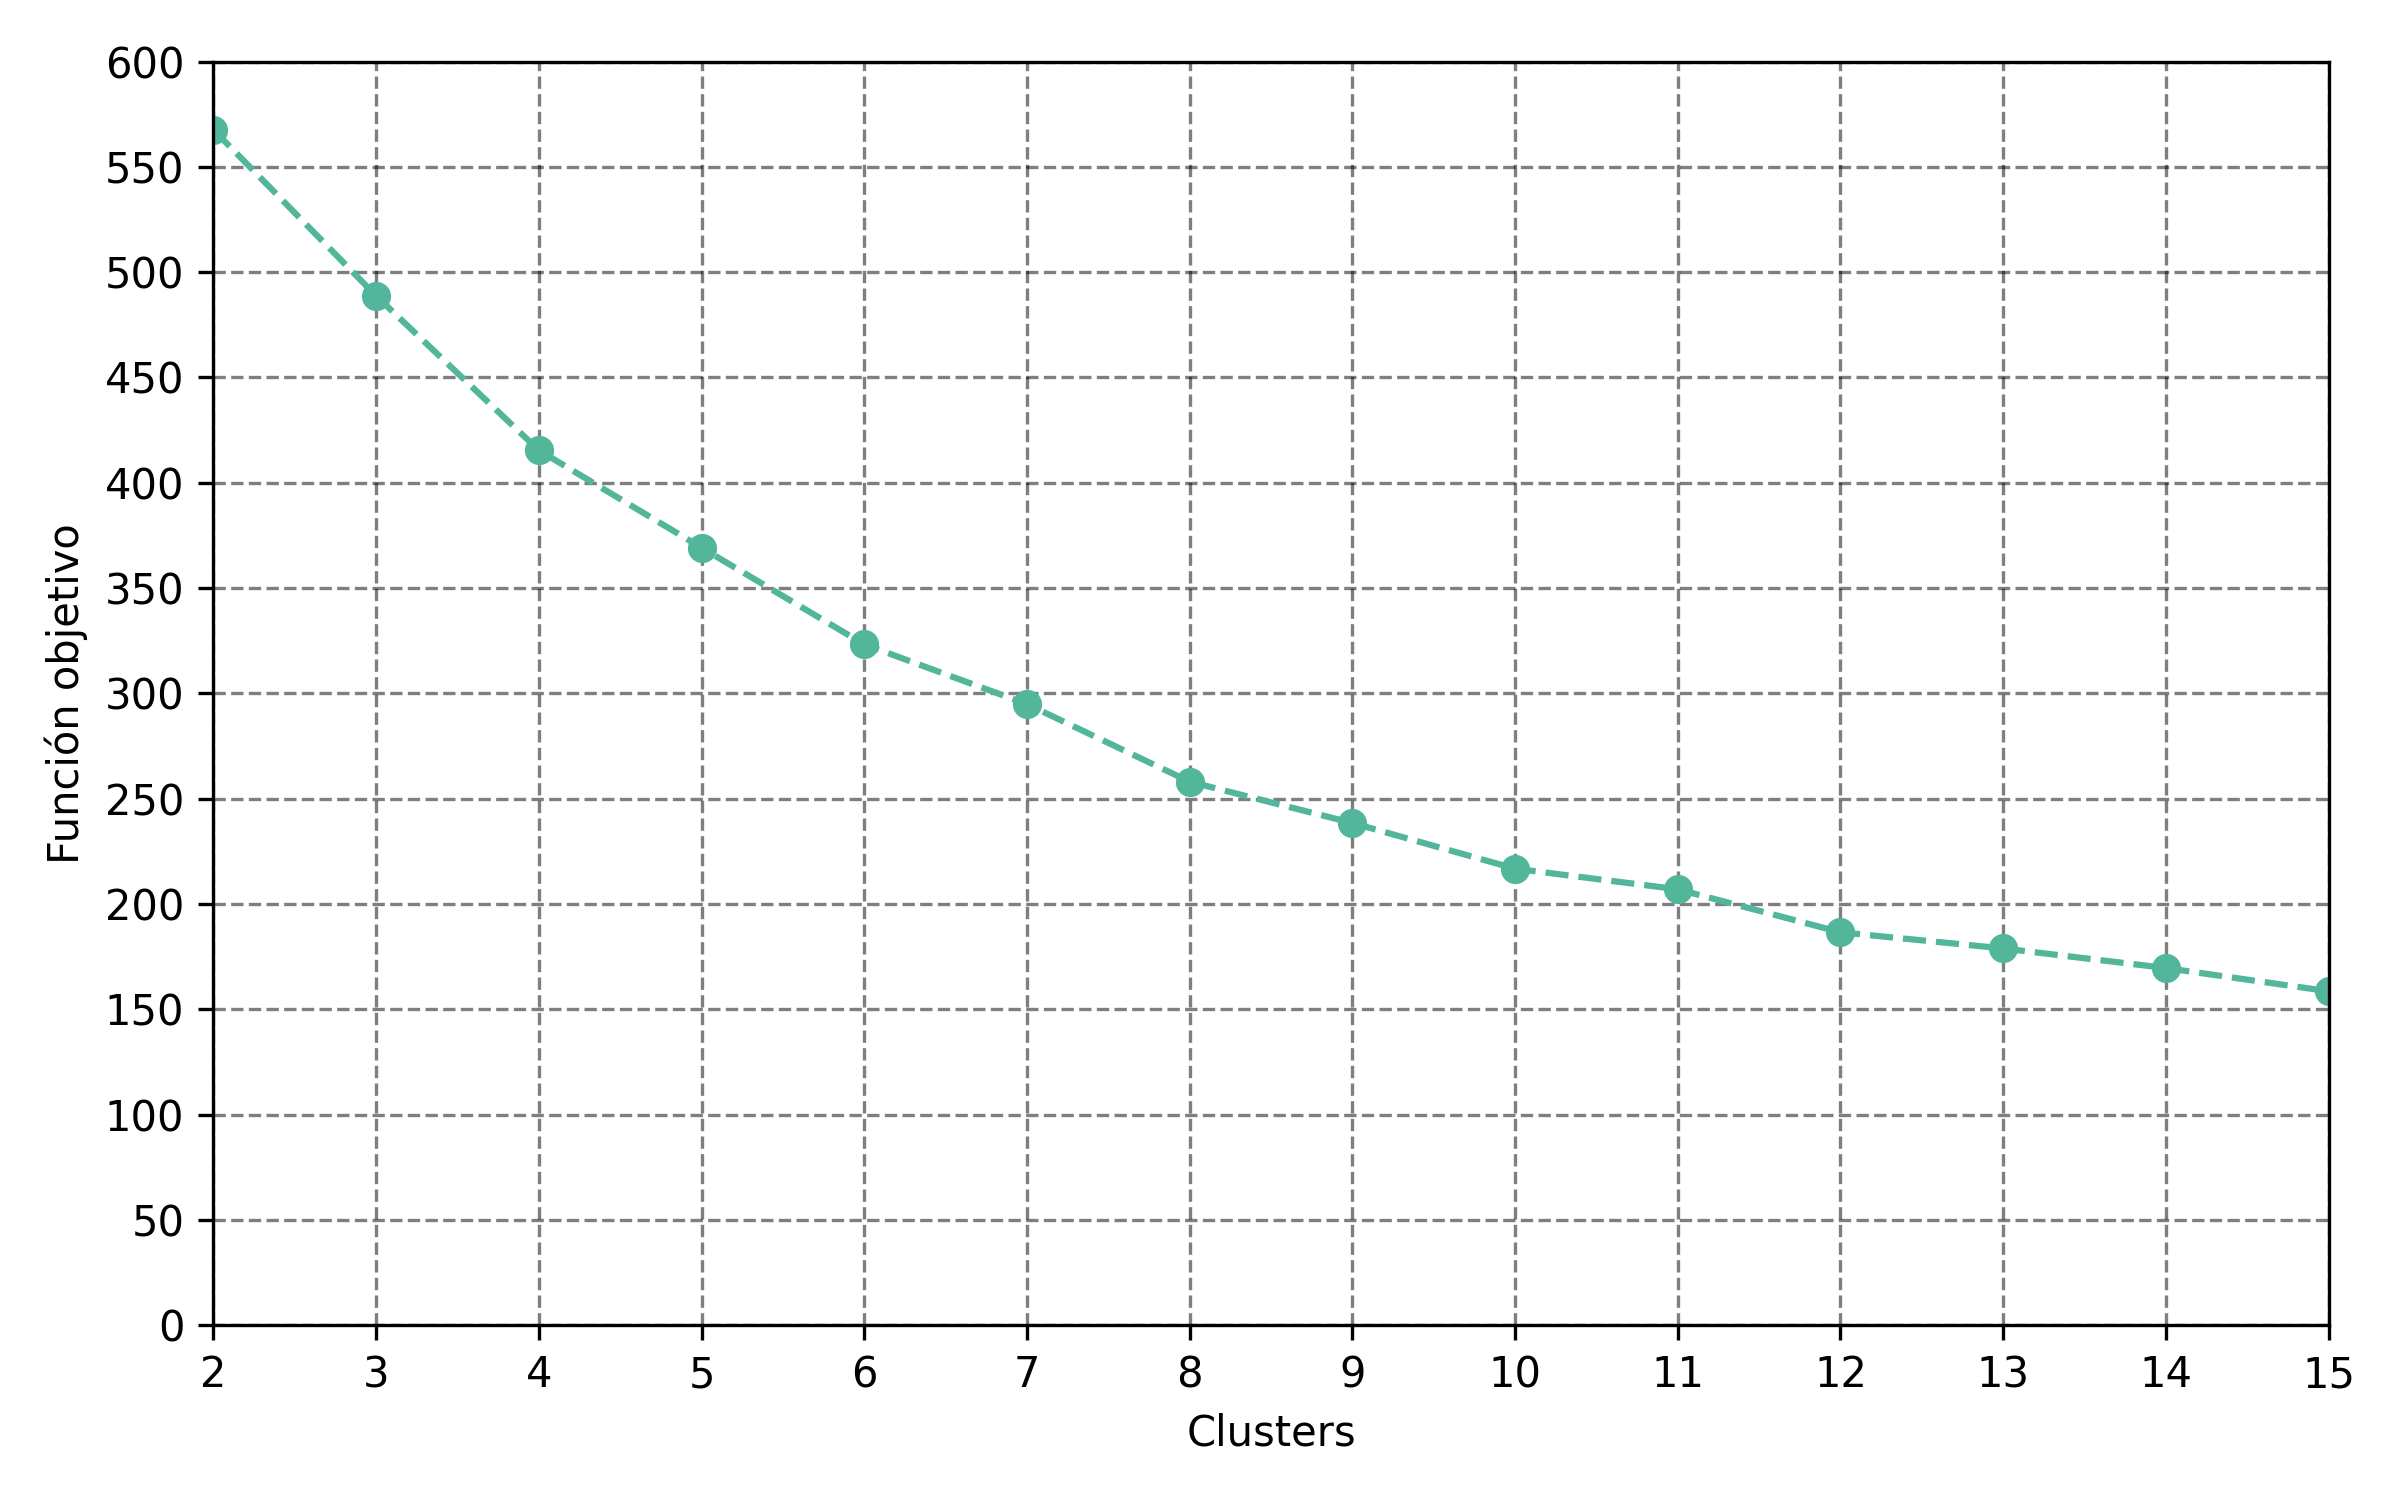
\includegraphics[width=14cm]{Graphics/Problema_03/train_scores.png}
    \caption{Valor de la función objetivo para los datos de entrenamiento.}
    \label{fig:problema_03_train_scores}
\end{figure}

El valor de k que seleccionaria de la gráfica sería 3. Esto debido a que el score obtenido tiene una diferencia con su anterior k mayor a comparación de las demás diferencias obtenidas.
\subsection*{Punto 02}

\textbf{Genere un conjunto de datos de validación del mismo tamaño que el conjunto de entrenamiento y de la misma manera. Para cada k, asigne cada punto o dato de validación a la media de clúster aprendida más cercana en la parte (a) y muestre en una gráfica el valor de la función objetivo resultante de k-medias usando los datos de validación como una función de k. Comenta lo que ves. Qué valor de k se seleccionaría si usara como criterio de selección el minimo valor de la funcion objetivo para los datos de validación?}
\subsection*{Punto 03}

\textbf{Para cada k, calcule y muestre en una gráfica el indice (score) Calinski Harabasz (CH) calculado para los datos de entrenamiento. Muestra CH como una función de k, y comente al respecto. Que valor de k maximiza este criterio?}

En la figura \ref{fig:problema_03_calinski_score} se muestran los scores obtenidos con el índice de Calinski Harabasz para los datos de entrenamieno y validación. Si se quisiera obtener un máximo del índice se tomaría a k=2. Esto debido a que en los datos de entrenamieno y validación en donde se presenta este criterio.

\begin{figure}[H]
    \centering
    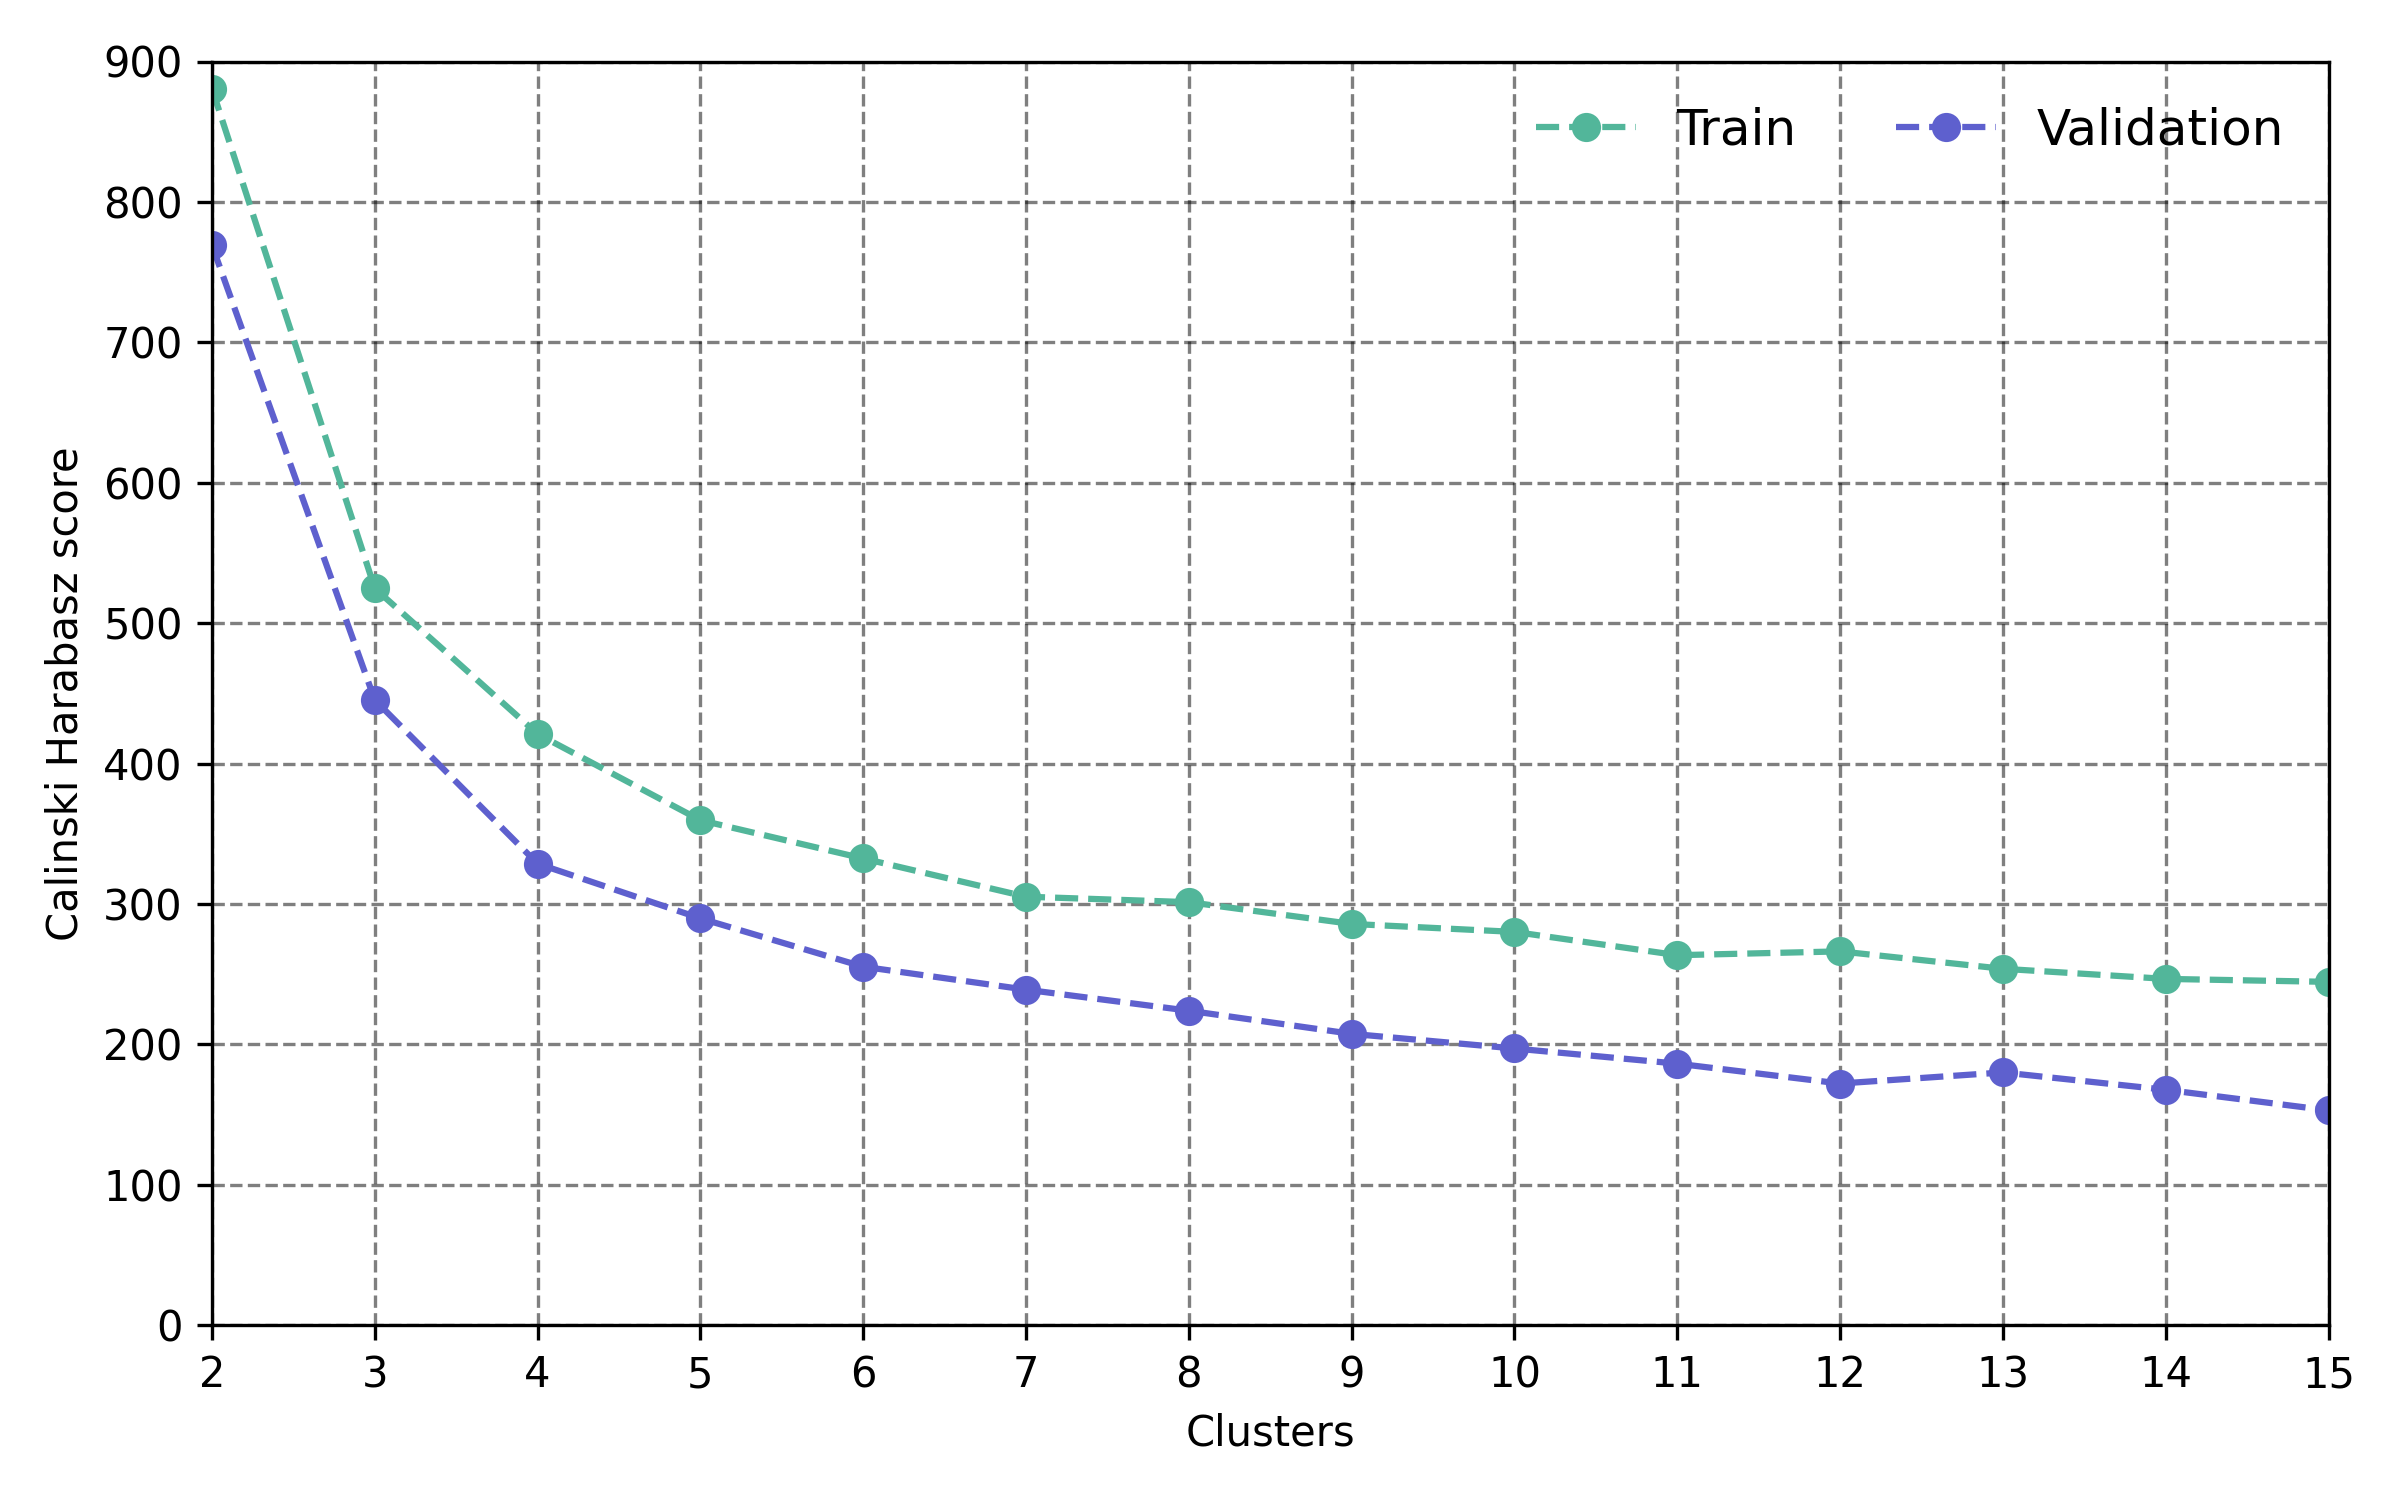
\includegraphics[width=15cm]{Graphics/Problema_03/calinski_harabasz_score.png}
    \caption{Índice de Calinski Harabasz obtenido a partir de la predicción de los datos de entrenamiento y validación.}
    \label{fig:problema_03_calinski_score}
\end{figure}



